%%%%%%%%%%%%%%%%%%%%%%%%%%%%%%%%%%%%%%%%%%%%%%%%%%%%%%%%%%%%%%%%%%%%%%%%%%%%%%%%%%%%%%%%%%%%%
%%									   Chapitre 3	    								 %%
%%%%%%%%%%%%%%%%%%%%%%%%%%%%%%%%%%%%%%%%%%%%%%%%%%%%%%%%%%%%%%%%%%%%%%%%%%%%%%%%%%%%%%%%%%%%%
\chapter{Modélisation statique et dynamique du système}
\minitoc
\newpage
%%%%%%%%%%%%%%%%%%%%%%%%%%%%%%%%%%%%%
\section{Introduction}
Un projet informatique nécessite une phase d'analyse et de modélisation. Dans la phase d'analyse, on cherche d'abord à bien comprendre et à décrire de façon précise les besoins des utilisateurs. Que souhaitent-ils faire avec le logiciel ? Quelles fonctionnalités veulent-ils ? Pour quel usage ? Comment l'action devrait-elle fonctionner ? C'est ce qu'on appelle « l'analyse des besoins ». 
\medskip

Nous allons dans ce chapitre faire en premier temps une modélisation orienté objet de notre système avec le langage UML (\glsentrylong{uml}) est ses outils : les diagrammes. Nous verrons comment ce langage contribue à la phase d'analyse des besoins et du domaines de notre projet. En deuxième temps, on va se servir de la méthode MERISE pour modéliser notre base données.

\section{Modélisation dynamique du système}
Pour ce qui est de la modélisation dynamique, on usera du formalisme UML (\glsentrylong{uml}) qu'on traduit par « Langage de Modélisation
Unifié ». UML est un méthode de modélisation visuel constitué d'un ensemble de schémas appelés des diagrammes, qui donnent chacun une vision différente du projet à traiter. En effet, ce dernier s'impose aujourd'hui, comme le langage de modélisation objet standardisé pour la conception des logiciels.

\subsection{Spécification des besoins}
La spécification des besoins est certainement l'étape qui ne doit pas être négligée. En effet, celle-ci permet de déterminer les fonctionnalités que chaque utilisateur attend de l'application.

\subsubsection{Les besoins des gestionnaires des ressources humaines}
Pour le gestionnaire, le logiciel doit permettre :
\begin{itemize}
	\item De gérer l'administration des employés : l'enregistrement, le suivi, le contrôle des données individuelles et la manipulation des renseignements du personnel.
	\item De gérer la gestion des rémunérations et de la paie : paiement des salaires, des primes.
	\item D'assurer la gestion des présences et des absences, des heures supplémentaires.
	\item D'alerter instantanément d'une nouvelle demande.
	\item De valider ou refuser les demandes de congés et d'avance.
	\item D'exporter les données.
	\item De créer des fiches employeur.
	\item D'archiver automatiquement les factures.
	\item De gérer les compétences et les diplômes des employés.
\end{itemize}

\subsubsection{Les besoins des responsables administratif scolarité}
Les responsables administratif scolarité veut un logiciel qui :
\begin{itemize}
	\item Gère les formations : création des mentions, parcours, salles de classes, niveaux et matières.
	\item Gère les emplois du temps.
	\item Automatise les tâches courantes : certificat de scolarité, carte étudiant, fiche d'inscription.
\end{itemize}

\subsubsection{Les besoins des salarié}
Les salariés sont composés par trois acteur : les simples employés, les enseignants et les chef de mention.
\medskip

Pour les employés, l'application doit leur permettre : 
\begin{itemize}
	\item De gérer leur agenda : ajout, modification, suppression et affichage des évènement.
	\item D'envoyer des demande d'absence, de congés, de remboursement ou d'avance.
	\item D'accéder et mettre à jour à ses informations personnelles et professionnelles (ajout de compétence, diplômes,...).
	\item De consulter leur emploi du temps personnel. 
	\item D'accéder à sa fiche de paie.
	\item De générer un CV (Curriculum Vitæ).
	\item D'envoyer un message
\end{itemize}
\medskip

Les chefs de mention veut une application :
\begin{itemize}
	\item Pour organiser les études académique : définition des Unités d'Enseignement (UE) , ses Éléments Constitutifs (EC) et le système de crédit du LMD. 
	\item Pour créer une promotion et affecter des étudiants dedans.
	\item Pour suivre les promotions en cours : commencer ou terminer un semestre, orientation des étudiants vers les spécialités.
	\item Qui permet de créer un profil de risque unique pour la population étudiante afin d'alerter les étudiants à risque d'échec.
\end{itemize}
\medskip

Pour le cas des enseignants, ils attend d'une application qui : 
\begin{itemize}
	\item Permet d'affecter les notes des étudiants pour son module.
	\item Permet de consulter les emplois du temps.
\end{itemize}
\medskip

Note : A savoir que l'acteur employé est une généralisation des deux acteurs chef de mention et enseignant, ce qui veut dire que les ces derniers ont accès à tous les taches des employés.

\subsubsection{Les besoins des étudiants}
Les attentes des étudiants du logiciel sont : 
\begin{itemize}
	\item Avoir une application haut niveau, interactives et intuitives avec facilité d'utilisation et accessible sur tout type de plateforme et enfin une architecture adaptative et configurable.
	\item Consulter les pré-requis d'obtention de semestre, année ou diplôme.
	\item Accéder à des bibliothèques de ressources universitaire en ligne.
	\item De communiquer entre étudiants.
\end{itemize}

\subsubsection{Les besoins de l'administrateur client}
En plus des tâches cités ci-dessus, l'administrateur client attend d'une application : 
\begin{itemize}
	\item Qui permet de gérer les utilisateur du logiciel : d'ajouter, modifier ou supprimer un utilisateur.
	\item Qui supporte l'envoie de message à tous les utilisateurs pendant une durée déterminée (avis de réunion, promotion, etc).
	\item Qui offre des notifications des éventuelles activités des personnels.
	\item Qui fait des suivis de l'établissement.
	\item Qui permet la gestion des locaux, logement, et les programmes de formation continue.
	\item Qui offre un tableau de bord orienté rôles qui affiche les chiffres clés et une vue d'ensemble de l'établissement.
	\item Qui permet de consulter et analyser les données par département et par programme.
\end{itemize}

\subsubsection{Les besoins du prestataire de l'application}
Pour le  prestataire, qui est l'administrateur de l'application SaaS.
\begin{itemize}
	\item Gestion des comptes clients et des utilisateurs.
	\item Gestion des abonnements : définir l'abonnement choisi par la société(le nombre d'utilisateur et les services ou modules choisis).
	\item Créer la base de données pour chaque nouvelle société client à partir d'une base de données de référence.
	\item Mise à jour et déploiement de l'application.
\end{itemize}
\medskip

\subsection{Diagrammes de cas d'utilisation}
Le diagramme de cas d'utilisation est un diagramme dédié à l'expression des besoins et à la description des processus. Il est utilisé pour donner une vision globale du comportement fonctionnel du système.
\medskip

Les diagrammes de cas d'utilisation qu'on montrer ici représentent les relations et les interactions intervenant dans notre système.
\medskip

Dans la partie gauche de chacun de ses diagramme de cas d'utilisation, sont figurés les acteurs primaires : les administrateurs, les gestionnaire RH (Ressources Humaines), les responsable de la scolarité, les enseignants et les chefs de mentions. Ceux sont les acteurs qui déclenchent les cas d'utilisation. 
\medskip

L'acteur secondaire, la base de données, est épargné pour ne pas encombrer les diagrammes, c'est l'acteur qui est sollicité par les cas d'utilisation.

%\newgeometry{top=2cm, bottom=2cm, left=0.5cm, right=0.5cm}



\clearpage
%\newgeometry{top=2.5cm, bottom=2cm, left=3cm, right=2.5cm, headheight=15pt}

\subsection{Diagrammes de séquences}
Elles sont la représentation graphique des interactions entre les acteurs et le système du point de vu dynamique qui nous montre le fonctionnement.
\medskip

Dans un souci de simplification, on représente l'acteur principal à gauche du diagramme, et l'acteur secondaire à droite du système. Le but étant de décrire comment se déroulent les actions entre les acteurs ou objets.
\medskip

La dimension verticale du diagramme représente le temps, permettant de visualiser l'enchaînement des actions dans le temps, et de spécifier la naissance et la mort d'objets.
\medskip

Avant d'entrer au menu et faire l'ensemble des autres scénarios, chaque utilisateur doit impérativement s'authentifier en utilisant son login et un mot de passe pour la sécurité du système.
\medskip

Le diagramme qui suit présente la phase d'authentification de chaque utilisateur.

\begin{figure}[h]
	\centering
	\includegraphics[width=1\linewidth]{"Chapitre3/images/sd/Authentification"}
	\caption{Diagramme de séquence : Authentification}
	\label{Diagramme de séquence : Authentification}
\end{figure}

\clearpage

Cette figure décrit les scénarios possibles lors de l'authentification utilisateur.

\begin{itemize}
	\item [\textgreater] L'utilisateur demande l'accès à l'application et donne le login et le mot de passe. 
	\item [\textgreater] Un test doit être réalisé (existence et compatibilité du login / mot de passe).
	\item [\textgreater] Si les données sont correctes alors permettre à l'internaute d'accèder à l'application.
	\item [\textgreater] Si les données ne sont pas correctes est pas valide, l'utilisateur doit soit réessayer, soit quitter l'application.
\end{itemize}
\medskip

Après l'authentification de l'utilisateur il y a tout un framework derrière, il valide l'authentification de dernier utilisateur connecter avec les droits qu'il a tout en récupérant ses derniers de la base de donnée.
\medskip

Tout au long de la session de l'utilisateur, il a la possibilité d'accéder qu'aux services dont il est autorisé. Dans le cas contraire il sera redirigé vers une page d'erreur 404.
\medskip

Le diagramme qui suit représente la gestion des habilitations.

\begin{figure}[h]
	\centering
	\includegraphics[width=1\linewidth]{"Chapitre3/images/sd/Gestion des habilitations"}
	\caption{Diagramme de séquence : Gestion des habilitations}
	\label{Diagramme de séquence : Gestion des habilitations}
\end{figure}

\clearpage

Nous allons représenter ici quelques scénarios basique dont les utilisateurs pourront faire avec le système. 

\begin{figure}[h]
	\centering
	\includegraphics[width=1\linewidth]{"Chapitre3/images/sd/Ajout d'utilsateur"}
	\caption{Diagramme de séquence : Ajout d'utilisateur}
	\label{Diagramme de séquence : Ajout d'utilisateur}
\end{figure}

\begin{figure}[h]
	\centering
	\includegraphics[width=1\linewidth]{"Chapitre3/images/sd/Modification"}
	\caption{Diagramme de séquence : Modification}
	\label{Diagramme de séquence : Modification}
\end{figure}

\begin{figure}[h]
	\centering
	\includegraphics[width=1\linewidth]{"Chapitre3/images/sd/Suppression"}
	\caption{Diagramme de séquence : Suppression}
	\label{Diagramme de séquence : Suppression}
\end{figure}

\begin{figure}[h]
	\centering
	\includegraphics[width=1\linewidth]{"Chapitre3/images/sd/Demandes"}
	\caption{Diagramme de séquence : Demandes de congé / absence / avance}
	\label{Diagramme de séquence : Demandes de congé / absence / avance}
\end{figure}

\clearpage

En principe tous les scénarios qui restent ont presque la même logique au niveau des interactions, par conséquent nous allons présenter le scenario qui décrit l'envoi de message par mail.
\medskip

\begin{figure}[h]
	\centering
	\includegraphics[width=1\linewidth]{"Chapitre3/images/sd/Envoi message"}
	\caption{Diagramme de séquence : Envoi un e-mail}
	\label{Diagramme de séquence : Envoi un e-mail}
\end{figure}

Des diagrammes d'activités peuvent aussi être utilisés comme des alternatives aux
diagrammes de séquence pour décrire un cas d'utilisation. Ils représente les règles d'enchaînement des actions et décisions au sein d'une activité, sous la forme d’un déroulement d'états regroupés séquentiellement comme un organigramme. Mais ils ne représentent pas les interactions entre les éléments du système et de ses acteurs contrairement aux diagrammes d'activités.

\section{Modélisation de la base de données}

\subsection{Définitions de la base de données}
Une base de données (\glsentryshort{bdd}) est un ensemble structuré de connaissance organisée à l'aide d'un formalisme. Elle représente les informations nécessaires au fonctionnement d'une entreprise \cite{bdMenja}. Ces données doivent pouvoir être utilisées par des utilisateur différents. Ainsi, la base de données est généralement couplée à celle de réseau, afin de pouvoir mettre en commun ces informations.

\begin{figure}[h]
	\centering
	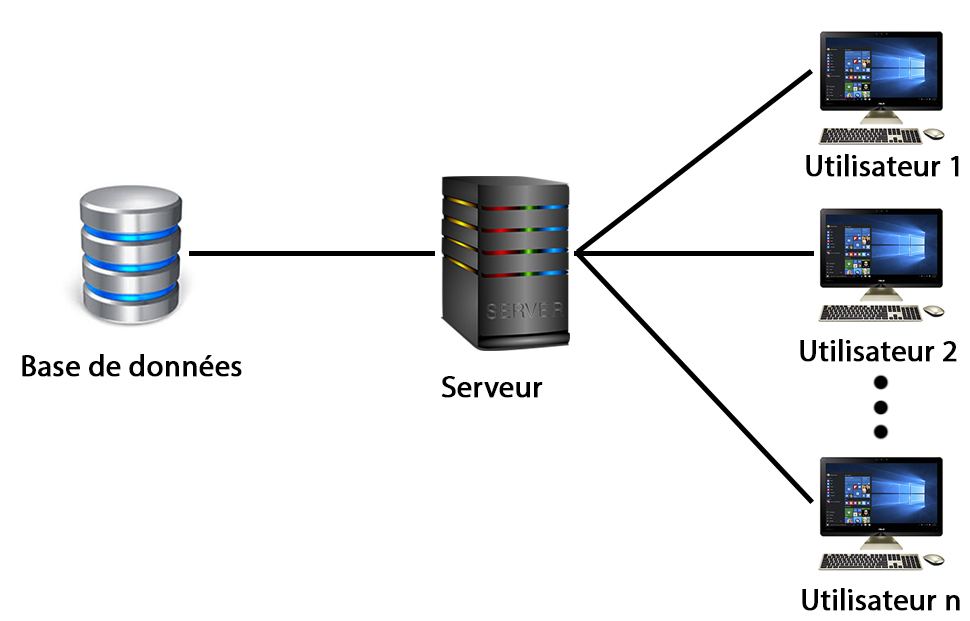
\includegraphics[width=0.8\linewidth]{Chapitre3/images/bd_system}
	\caption{Le système de la base de données}
	\label{Le système de la base de données}
\end{figure}

\subsection{Modélisation MERISE}
On a besoin de modéliser une base de données \cite{bdMenja} : 
\begin{itemize}
	\item Pour définir le contenu en informations (connaissances) de la future base de données.
	\item Le modèle en tant que tel est un résultat scientifique car décrit et résume le "savoir" disponible sur un sujet à un instant donné.
	\item Pour disposer d'un outil de communication accessible aux futurs utilisateur de la base de données.
\end{itemize}

Pour ce qui est de la modélisation de la base de données, nous utiliserons la méthode de MERISE, qui est une méthode d'analyse de conception des systèmes d'information basée sur le principe de la séparation des données et des traitements \cite{merise}. Elle possède un certain nombre de modèles (ou schémas) qui sont répartis sur 3 niveaux : 
\begin{itemize}
	\item Le niveau conceptuel : contenu de la base en termes de concepts (Modèle Entité Association), 
	\item Le niveau logique ou organisationnel : traduction du schéma conceptuel dans le paradigme du système de base de données (modèle relationnel), 
	\item Le niveau physique : organisation et accès aux données dans la base.
\end{itemize}

Nous ne nous intéresserons ici qu'à certaines schémas permettant la conception d'une base de données relationnelle.

\subsection{Le dictionnaire des données}
Le dictionnaire des données est un documents qui regroupe toutes les données que vous aurez à conserver dans votre base. Pour chaque donnée, il indique : 
\begin{itemize}
	\item Le code mnémonique : il s'agit d'un libellé désignant une donnée.
	\item La désignation : il s'agit d'une mention décrivant ce à qui la donnée correspond.
	\item La nature de donnée : 
	\begin{itemize}
		\item [\textbullet] A ou Alphabétique : lorsque la donnée est uniquement composée de caractères alphabétique.
		\item [\textbullet] N ou Numérique : lorsque la donnée est composée uniquement de nombres (entiers ou réels).
		\item [\textbullet] AN ou Alphanumérique : lorsque la donnée peut être composée à la fois de caractères alphabétiques et numériques.
		\item [\textbullet] Date : lorsque la donnée est une date (au format AAAA-MM-JJ)
		\item [\textbullet] Booléen : Vrai ou Faux
	\end{itemize}
	\item La taille : elle s'exprime en nombre de caractères ou de chiffres.
	\item Le type de donnée :
	\begin{itemize}
		\item [\textbullet] E : Élémentaire;
		\item [\textbullet] Ca : Résultat d'un calcul ;
		\item [\textbullet] Co : Résultat d'une concaténation.
	\end{itemize}
\end{itemize}

\clearpage
Voici le tableau montrant le dictionnaire de données importantes de notre base de données.

\begin{center}
	{\renewcommand{\arraystretch}{1.5} % horizontal padding
		\setlongtables		
			\begin{longtable}{|c|>{\centering}m{7cm}|c|c|}
		
				% Entête de la première page
				\caption{Dictionnaire de données}
				\label{Dictionnaire de données}
				\endfirsthead
				
				% Entête de toutes les pages
				\hline \textbf{Propriété} & \textbf{Contenu} & \textbf{Nature} & \textbf{Taille}\\
				\hline
				\endhead
				
				% Bas de toutes les pages
				\endfoot
				
				% Contenu du tableau

				\hline \textbf{Propriété} & \textbf{Contenu} & \textbf{Nature} & \textbf{Taille}\\
				
				\hline id\_util & Identifiant de l'utilisateur & N & 10 \\ 
				\hline nom\_util & Nom de l'utilisateur & A & 30 \\ 
				\hline prenom\_util & Prénom de l'utilisateur & A & 60 \\ 
				\hline sexe\_util & Sexe de l'utilisateur & A & 10 \\ 
				\hline date\_naissance & Date de naissance de l'utilisateur & Date & - \\
				\hline adresse\_util & Adresse utilisateur & AN & 120 \\
				\hline etat\_civil & Etat civil de l'utilisateur & AN & 30 \\
				\hline tel\_util & Numéro de téléphone de l'utilisateur & N & 15 \\
				\hline email\_util & Adresse email de l'utilisateur & AN & 60 \\
				\hline nation\_etu & Nationalité de l'étudiant & A & 30 \\
				\hline cin\_etu & Numéro carte d'identité national de l'utilisateur & N & 12 \\
				\hline photo & Numéro carte d'identité national de l'étudiant & AN & 30 \\
				
				\hline id\_par & Identifiant d'un parent & N & 10 \\
				\hline nom\_par & Nom d'un parent & A & 30 \\
				\hline prenom\_par & Prenom d'un parent & A & 60 \\
				\hline adresse\_par & Adresse d'un parent & AN & 120 \\
				\hline fonction\_par & Fonction d'un parent & A & 60 \\
				
				\hline id\_empl\_par & Identifiant de l'employé & N & 10 \\
				\hline grade & Grade d'un enseignant & A & 30 \\ 
				\hline date\_embauche & Date d'embauche de l'employé & Date & - \\
				\hline fonction\_empl & Fonction de l'employé & A & 60 \\
				
				\hline id\_dmd & Identifiant d'une demande & N & 10 \\
				\hline type\_dmd & Type d'une demande & A & 30 \\
				\hline contenu\_dmd & Contenu de la demande & AN & - \\
				
				\hline identifiant & Identifiant d'une authentification & AN & 30 \\
				\hline mdp & Mot de passe & AN & 60 \\
				\hline privilege & Droit d'accès de l'utilisateur & A & 30 \\
				
				\hline id\_mail & Identifiant d'un mail & N & 10 \\
				\hline destinataire & Destinataire du mail & AN & 60 \\
				\hline objet & Objet du mail & AN & 60 \\
				\hline contenu & Contenu du mail & AN & - \\
				
				\hline id\_admin & Identifiant de l'administrateur & N & 10 \\
				
				\hline nom\_eta & Nom de l'établissemant & AN & 30 \\
				\hline apropos\_eta & Apropos de l'établissement & AN & - \\
				
				\hline id\_doc & Identifiant d'un document & N & 10 \\
				\hline titr\_doc & Titre du document & AN & 60 \\
				\hline description\_doc & Description du document & AN & - \\
				             
				\hline id\_ensgn & Identifiant de l'enseignant & N & 10 \\
				\hline grade & Grade de l'enseignant & A & 30 \\
				
				\hline id\_etu & Identifiant de l'étudiant & N & 10 \\
				\hline date\_inscription & Date d'inscription de l'étudiant & Date & - \\
				
				\hline note & Note correspondante à une matière & N & 10 \\
				
				\hline id\_matiere & Identifiant d'une matière & N & 10 \\
				\hline designation & Nom de la matière & A & 60 \\
				\hline UE & Unité d'enseignement & A & 30 \\
				\hline coeff & Coefficient de la matière & N & 10 \\
				
				\hline id\_stage & Identifiant du stage & N & 10 \\
				\hline date\_debut & Date de début du stage & Date & - \\
				\hline date\_fin & Date de fin du stage & Date & - \\
				
				\hline id\_theme & Identifiant d'un thème & N & 10 \\
				\hline nom\_thme & Nom d'un thème & AN & 120 \\
				
				\hline nom\_mention & Nom d'une metion ou département & A & 120 \\
				
				\hline id\_parcours & Identifiant du parcours ou de la filière & N & 10 \\
				\hline nom\_parcours & Nom du parcours & A & 120 \\
				
				\hline id\_classe & Identifiant d'une classe & N & 10 \\
				\hline nom\_classe & Nom d'une classe & AN & 120 \\
				
				\hline id\_niveau & Identifiant d'un niveau & N & 10 \\
				\hline nom\_niveau & Nom d'un niveau & AN & 30 \\
				
				\hline
				
			\end{longtable} 
	} \quad
\end{center}

\subsection{Le Modèle Conceptuel de Données (MCD)}
Le \gls{mcd} a pour but d'écrire de façon formelle les données
qui seront utilisées par le système d'information. Il s'agit donc d’une représentation sous forme d'un schéma des données relatives au sujet à traiter (en gros les entités, leurs attributs et les relations qu'elles entretiennent). (Voir figure 3.14).


\subsection{Le Modèle Logique de Données (MLD)}
L'étape du \gls{mld} se situe chronologiquement juste après l'étape MCD et revient à présenter les objets du MCD sous une forme compréhensible par un SGBD. Pour faire court, dans un contexte SGBD relationnel, les objets représentés sont
désormais des tables (disons SQL) et les liens qui les unissent. (Voir figure 3.15).

\newpage

\begin{landscape}
	\begin{figure}[h]
		\vspace*{-0.5cm}
		\centering
		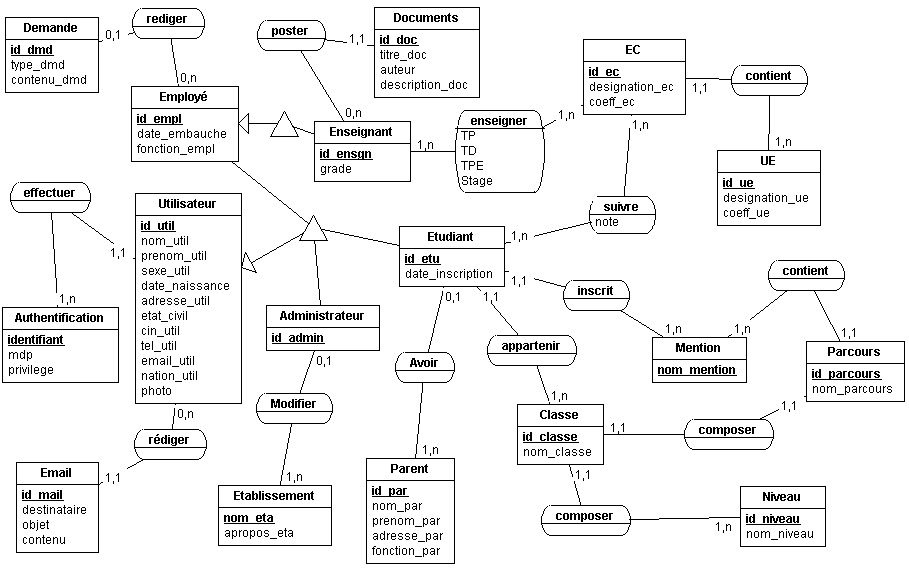
\includegraphics[width=1\linewidth]{Chapitre3/images/merise/MCD}
		\caption{Modèle Conceptuel de Données}
		\label{Modèle Conceptuel de Données}
	\end{figure}	
\end{landscape}

\newpage

\begin{landscape}
	\begin{figure}[h]	
		\vspace*{-1cm}
		\centering
		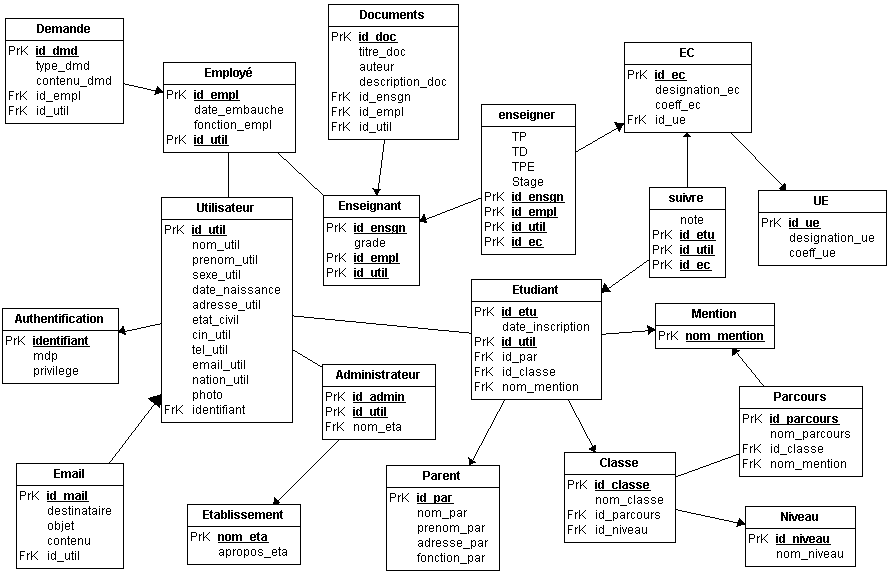
\includegraphics[width=1\linewidth]{Chapitre3/images/merise/MLD}
		\caption{Modèle Logique de Données}
		\label{Modèle Logique de Données}
	\end{figure}	
\end{landscape}

\section{Conclusion}
Dans ce chapitre, nous avons entamé la modélisation du logiciel. La conception et la modélisation sont supposées comme les noyaux du travail. En effet, celles-ci sont garantes que le système aboutira aux résultats espérés. Nous avons choisi UML comme langage de modélisation dynamique et MERISE pour la conception de la base de données. Le chapitre
suivant sera consacré à la programmation et la réalisation de l'application.